\documentclass[11pt]{article}

\usepackage[a4paper,margin=1in]{geometry}
\usepackage[T1]{fontenc}
\usepackage[utf8]{inputenc}
\usepackage{lmodern}
\usepackage{setspace}
\usepackage{amsmath}
\usepackage{booktabs}
\usepackage{array}
\usepackage{graphicx}
\usepackage{float}
\usepackage{hyperref}
\usepackage{caption}
\usepackage{xcolor}

\hypersetup{
  colorlinks=true,
  linkcolor=black,
  urlcolor=blue,
  pdftitle={Digital Payments and UPI in India: Structural Changes or Just Growth?},
  pdfauthor={Student Name}
}

\setstretch{1.08}
\setlength{\parskip}{0.5em}
\setlength{\parindent}{0pt}
\captionsetup{font=small}

\newcommand{\pp}{\text{ pp}}

\begin{document}

\begin{titlepage}
\centering
{\Large Statistical Inference Project Report\par}
\vspace{2.4cm}
{\huge\bfseries Digital Payments and UPI in India:\\[0.25cm] Structural Changes or Just Growth?\par}
\vspace{2.2cm}
{\large Prepared for: Statistical Inference\par}
\vspace{0.8cm}
{\large Department / Course: BS in Mathematics and Computing\par}
\vspace{0.8cm}
{\large Submitted by: Nitin Ekka\par}
\vspace{0.8cm}
{\large Roll Number(s): 22MA10039\par}
\vfill
{\large Date: April 16, 2026\par}
\end{titlepage}

\begin{abstract}
This report asks whether India's UPI expansion is only a story of rising levels or also a story of changing growth dynamics. The analysis combines two live data sources: the official Reserve Bank of India (RBI) monthly \emph{Payment System Indicators} archive and a machine-readable daily payments panel that is first validated against the official monthly archive before use. The daily panel covers June 1, 2020 to July 31, 2025, while the official monthly archive extends to December 2025. Monthly UPI volume and value growth are compared across two periods, pre-2022 and 2022 onward, using bootstrap confidence intervals, Welch two-sample tests, Mann--Whitney tests, and seasonality-adjusted regressions with HAC standard errors. The central result is that UPI continues to expand strongly in levels, but monthly percentage growth is materially lower after January 2022. Mean monthly volume growth falls from 7.28\% to 3.65\%, and mean monthly value growth falls from 6.80\% to 2.81\%. October and December remain important seasonal months in growth regressions, but a coarse festival-month dummy is not significant in level regressions. Daily autocorrelation patterns further justify robust inference. The correct interpretation is therefore not stagnation, but maturation on a much larger transaction base.
\end{abstract}

\section{Introduction}

UPI has become the dominant retail digital payments infrastructure in India. Its scale is now large enough that percentage growth and absolute growth can tell different stories. A mature payment system may still add very large numbers of transactions every month even while its growth rate slows. This report studies whether the Indian UPI trajectory after 2021 reflects a structural moderation in growth, or whether the apparent slowdown is simply noise around continued expansion.

The empirical questions are straightforward. First, has the average monthly growth rate of UPI transaction volume and value changed between the earlier diffusion phase and the later mature phase? Second, are festival months statistically different from non-festival months? Third, do the results survive basic seasonality controls and serial-correlation-aware inference? Finally, what does the daily data add that cannot be seen from monthly aggregates alone?

\section{Data Sources and Validation}

The primary official source is RBI's monthly \emph{Payment System Indicators} archive.\footnote{\url{https://www.rbi.org.in/Scripts/PSIUserView.aspx?Id=47}} The institutional background for UPI comes from a Press Information Bureau (PIB) explainer,\footnote{\url{https://www.pib.gov.in/PressReleaseIframePage.aspx?PRID=2079544}} while RBI's Database on Indian Economy (DBIE) is a supplementary official reference for payments statistics.\footnote{\url{https://data.rbi.org.in}} In addition, a machine-readable daily payments datastore is used for high-frequency robustness after direct validation against the official monthly archive.

The full reproducibility package for this report, including code, cleaned datasets, figures, notebook, and submission files, is available at \url{https://github.com/brownhat16/exercise2}.

The daily panel contains deduplicated UPI observations from June 1, 2020 through July 31, 2025. Daily UPI volume is reported in lakh transactions and daily UPI value in crore rupees. Aggregating the deduplicated daily panel to months reproduces the official RBI monthly UPI totals with mean absolute percent differences of essentially zero in overlapping months from June 2021 through July 2025. This validation step is important because it lets the daily data support the inference rather than substitute for the official archive.

\begin{figure}[H]
\centering
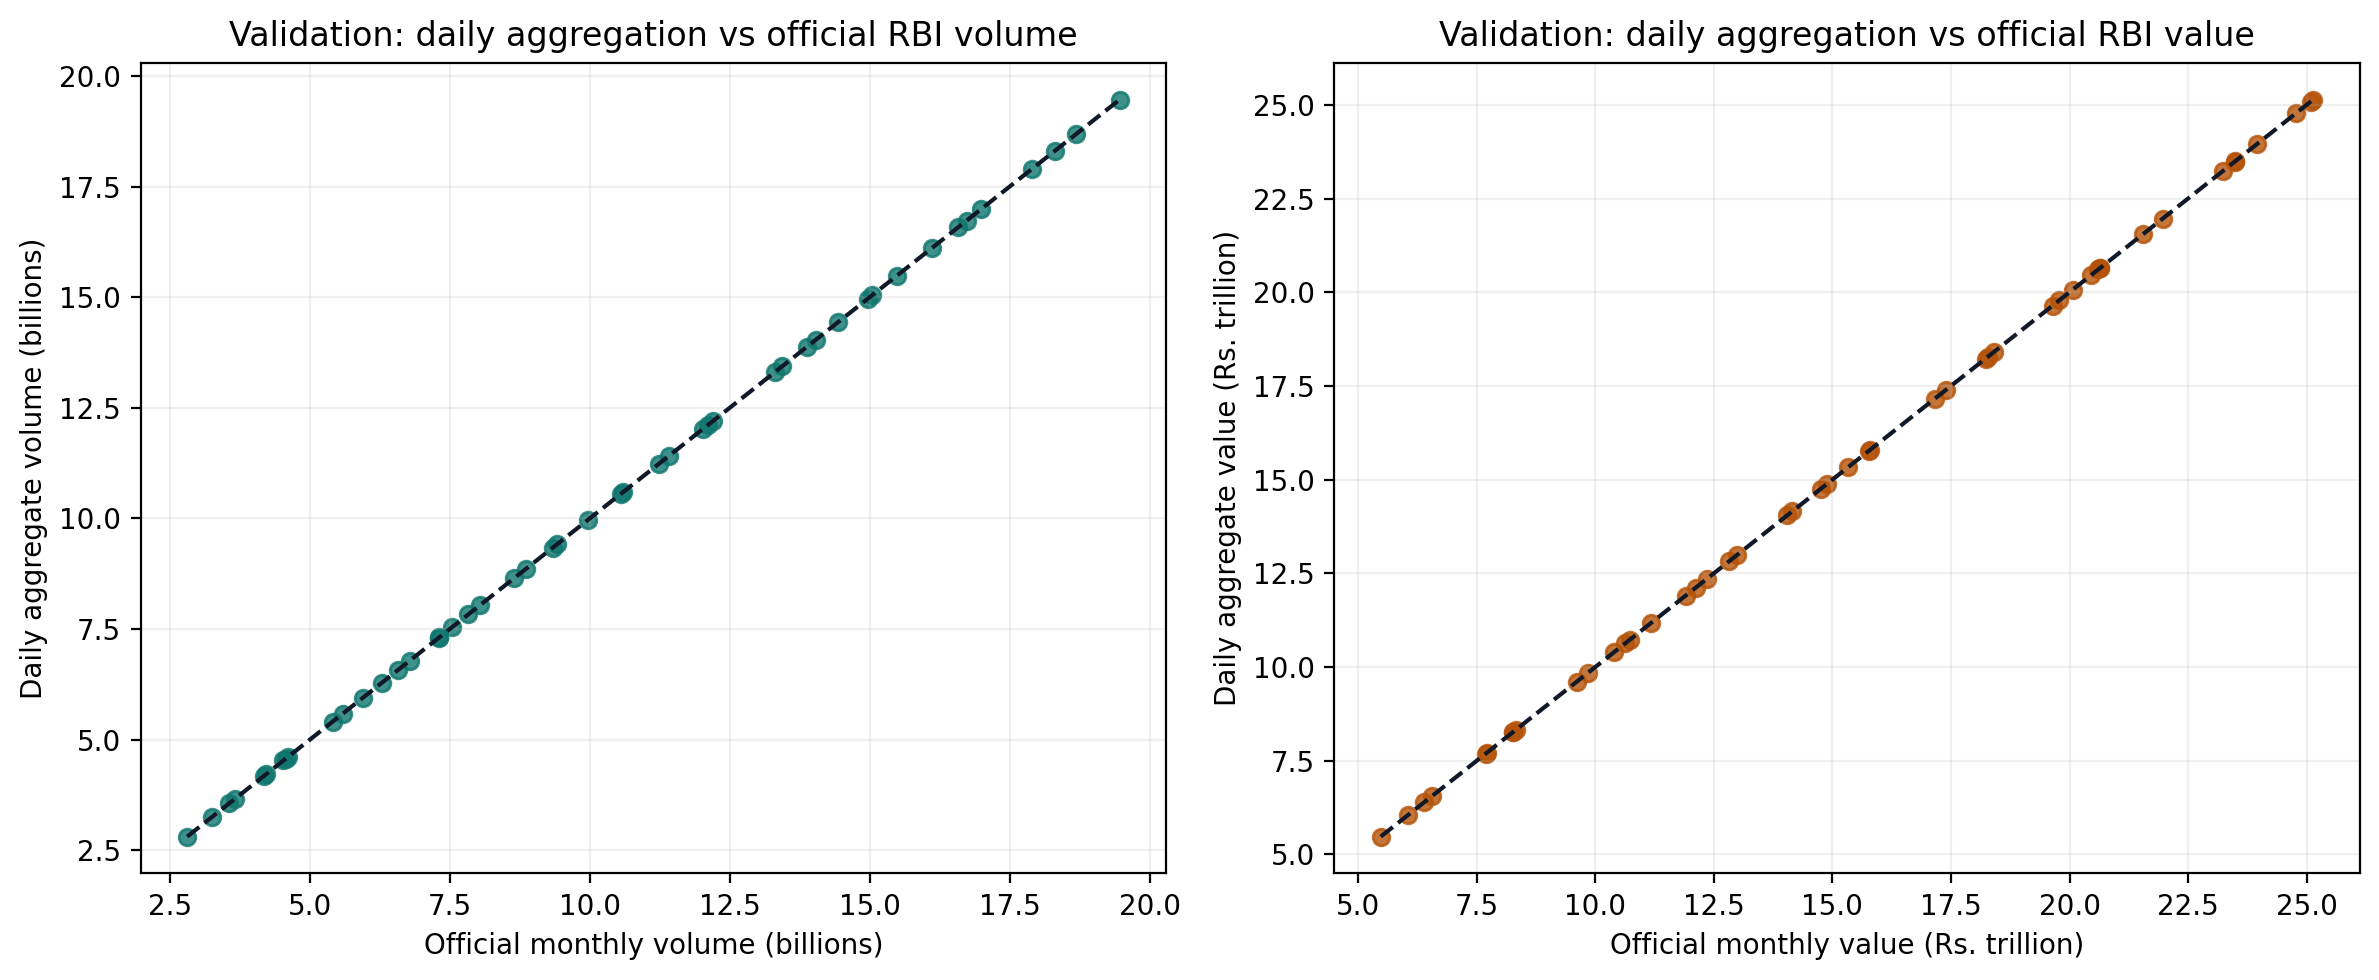
\includegraphics[width=0.94\textwidth]{upi_plot_validation_scatter.png}
\caption{Validation of monthly totals: daily aggregation versus official RBI monthly archive. The near-45-degree fit confirms that the machine-readable daily panel can be used for robustness after deduplication.}
\label{fig:validation}
\end{figure}

For the main statistical analysis, monthly data from June 2020 to July 2025 are used, with growth rates defined from July 2020 onward. The official archive is then used to extend level tracking through December 2025 for current context. The latest official month available in this run is December 2025, with UPI volume of 216{,}346.68 lakh transactions and UPI value of Rs.\ 2{,}796{,}713 crore. That is roughly 21.63 billion transactions and Rs.\ 27.97 trillion in a single month.

\section{Variable Construction and Empirical Design}

Monthly UPI volume and value are obtained by summing validated daily observations within each calendar month. The main outcome variables are monthly growth rates:
\[
g_t = 100\left(\frac{y_t}{y_{t-1}} - 1\right),
\]
where $y_t$ is monthly UPI volume or value. Two growth variables are therefore constructed: monthly volume growth and monthly value growth.

The main period split is:
\begin{itemize}
  \item \textbf{Pre-2022 period:} July 2020 to December 2021.
  \item \textbf{2022 onward period:} January 2022 to July 2025.
\end{itemize}

Festival months are coded as October, November, and December. This is a deliberately simple proxy and does not fully capture shifting festival dates such as Diwali, but it is sufficient for a first-pass seasonality comparison.

The estimation strategy has four layers:
\begin{enumerate}
  \item Bootstrap confidence intervals for the mean monthly growth rate in each period.
  \item Welch two-sample tests and Mann--Whitney tests for pre/post growth differences.
  \item OLS growth regressions with month dummies and HAC standard errors:
  \[
  g_t = \alpha + \beta \,\text{Post2022}_t + \sum_{m=2}^{12}\gamma_m D_{m,t} + \varepsilon_t.
  \]
  \item Trend-plus-festival regressions in log levels:
  \[
  \log(y_t) = \alpha + \delta t + \theta \,\text{Festival}_t + u_t.
  \]
\end{enumerate}

Because payment series are serially correlated, HAC standard errors are used instead of naive OLS standard errors. As a course-connected robustness exercise, annual averages of monthly growth are also reported because they are closer to independent observations than monthly growth itself.

\section{Main Results}

\subsection{Pre-2022 versus 2022 onward}

Table~\ref{tab:period-tests} reports the main pre/post comparison. The result is a clear moderation in growth after January 2022. Mean monthly UPI volume growth falls from 7.28\% to 3.65\%, a decline of 3.63 percentage points. Mean monthly UPI value growth falls from 6.80\% to 2.81\%, a decline of 3.99 percentage points.

\begin{table}[H]
\centering
\caption{Monthly growth comparison across periods}
\label{tab:period-tests}
\small
\begin{tabular}{p{3.4cm}p{3.0cm}p{3.0cm}c c c}
\toprule
Measure & Pre-2022 mean [95\% CI] & 2022 onward mean [95\% CI] & Post $-$ pre & Welch $p$ & Mann--Whitney $p$ \\
\midrule
UPI volume growth & 7.28\% [4.05, 10.54] & 3.65\% [2.03, 5.36] & $-3.63\pp$ & 0.062 & 0.046 \\
UPI value growth & 6.80\% [3.76, 9.98] & 2.81\% [1.23, 4.42] & $-3.99\pp$ & 0.036 & 0.056 \\
\bottomrule
\end{tabular}
\end{table}

The value-growth slowdown is statistically significant under Welch's unequal-variance test. The volume-growth slowdown is marginal under Welch's test but significant under the Mann--Whitney alternative, which is consistent with non-Gaussian and potentially heavy-tailed monthly growth. The joint reading is that growth has moderated materially even though the system continues to expand.

\begin{figure}[H]
\centering
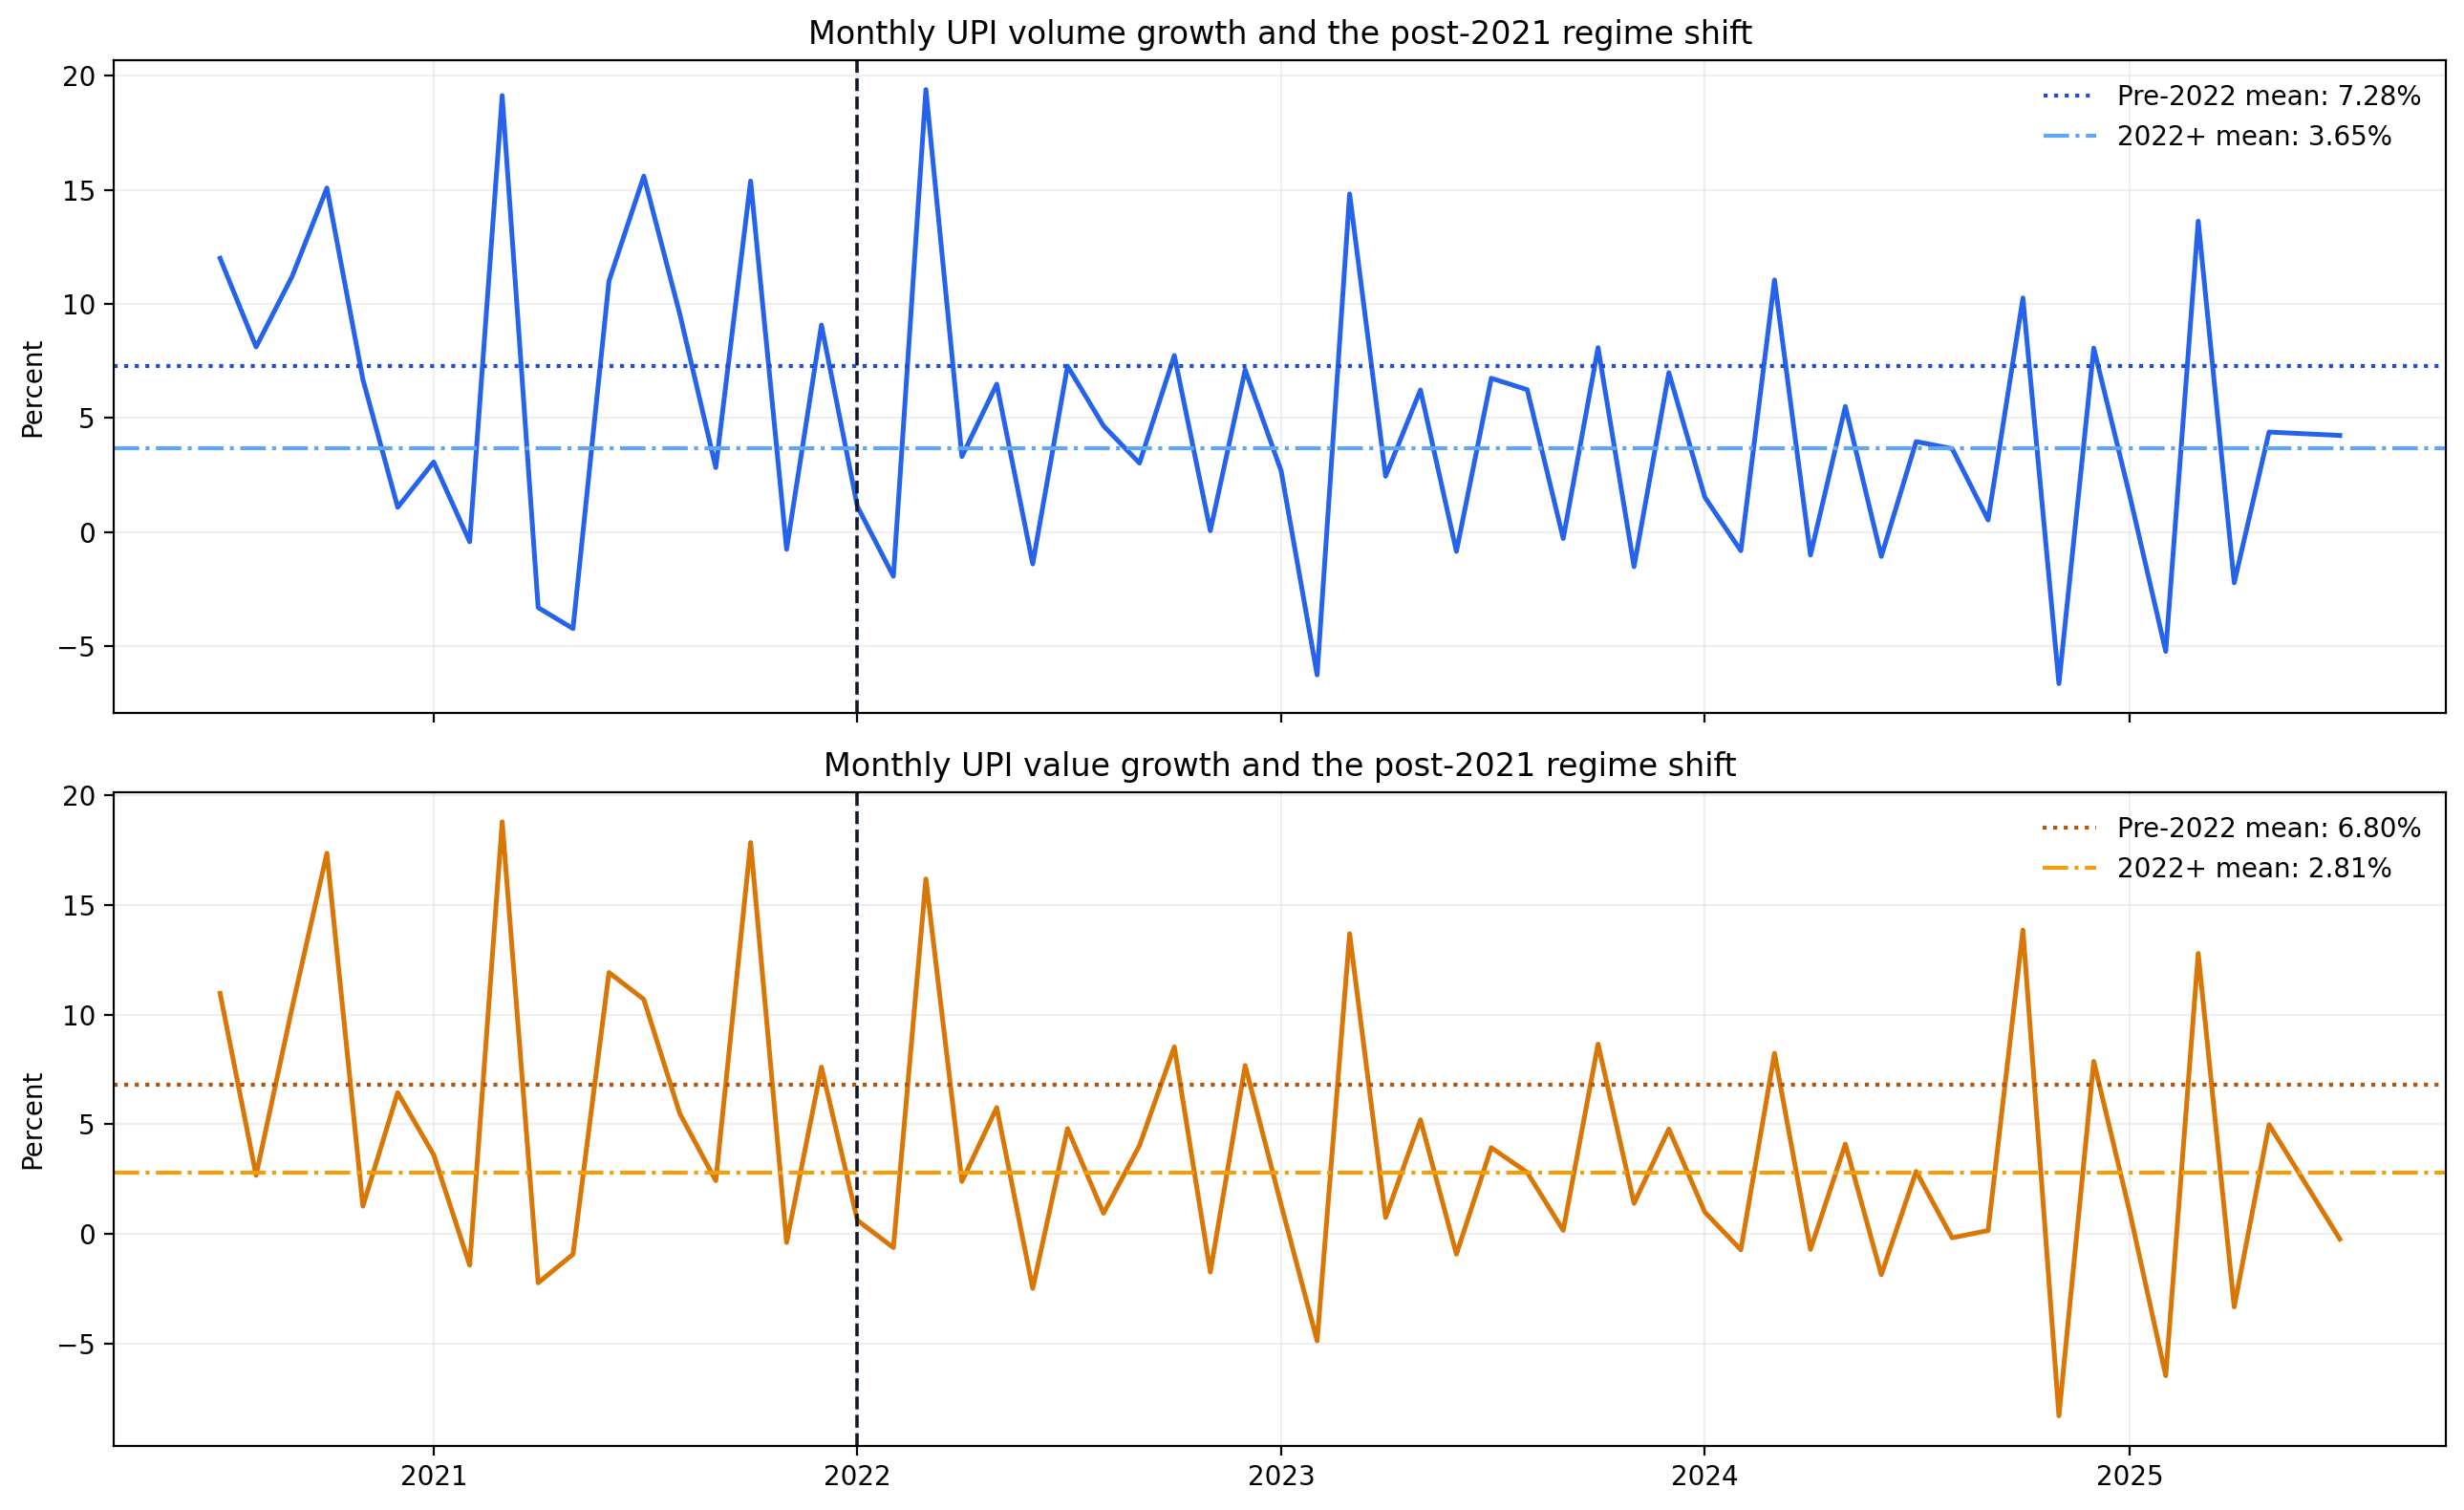
\includegraphics[width=\textwidth]{upi_plot_growth_regime.png}
\caption{Monthly UPI growth in volume and value with the January 2022 break marked explicitly. The dashed line separates the diffusion phase from the mature phase, while horizontal reference lines show lower average growth after 2021.}
\label{fig:growth-regime}
\end{figure}

\subsection{Festival-month comparisons}

Naive festival-month comparisons in levels are weak. Festival-month Welch $p$-values are 0.861 for volume and 0.931 for value, while the corresponding log-level tests are also far from significance. This does not imply an absence of seasonality. It implies that a coarse October--December dummy is not enough, by itself, to separate trend from seasonal effects in levels.

\subsection{Seasonality-adjusted regression evidence}

The growth regressions are more informative because they separate post-2021 structural change from regular calendar variation. Table~\ref{tab:regression-results} summarizes the key coefficients.

\begin{table}[H]
\centering
\caption{Growth regressions with HAC standard errors}
\label{tab:regression-results}
\small
\begin{tabular}{l l r r r}
\toprule
Model & Term & Coefficient & HAC s.e. & $p$-value \\
\midrule
Volume growth & Post-2022 indicator & -3.3031 & 0.9715 & 0.0007 \\
Volume growth & October & 8.6544 & 0.9941 & $<0.001$ \\
Volume growth & November & -3.0915 & 1.6893 & 0.067 \\
Volume growth & December & 3.8068 & 1.4447 & 0.008 \\
Value growth & Post-2022 indicator & -3.7421 & 0.7232 & $<0.001$ \\
Value growth & October & 10.9807 & 1.2075 & $<0.001$ \\
Value growth & November & -3.8076 & 1.4683 & 0.010 \\
Value growth & December & 4.6124 & 0.8028 & $<0.001$ \\
\bottomrule
\end{tabular}
\end{table}

The post-2022 coefficient remains strongly negative in both growth regressions, which is the cleanest evidence for structural moderation. October is the strongest positive seasonal month in both volume and value growth, and December is also significantly positive. November is weaker and partly negative, suggesting that the timing of holiday-related spending and settlement is more nuanced than a simple quarter-end festival dummy can capture.

\subsection{Trend-plus-festival regressions}

In log-level regressions with a deterministic trend, the monthly trend remains strongly positive:
\begin{itemize}
  \item log-volume trend coefficient: 0.0425 per month,
  \item log-value trend coefficient: 0.0359 per month.
\end{itemize}

However, the coarse festival-month coefficient is not statistically distinguishable from zero:
\begin{itemize}
  \item log-volume festival coefficient: 0.0509, $p=0.247$,
  \item log-value festival coefficient: 0.0492, $p=0.320$.
\end{itemize}

This again supports the interpretation that the dominant feature of the data is strong trend, while finer month-specific seasonality is better captured by explicit month dummies than by a broad festival indicator.

\begin{figure}[H]
\centering
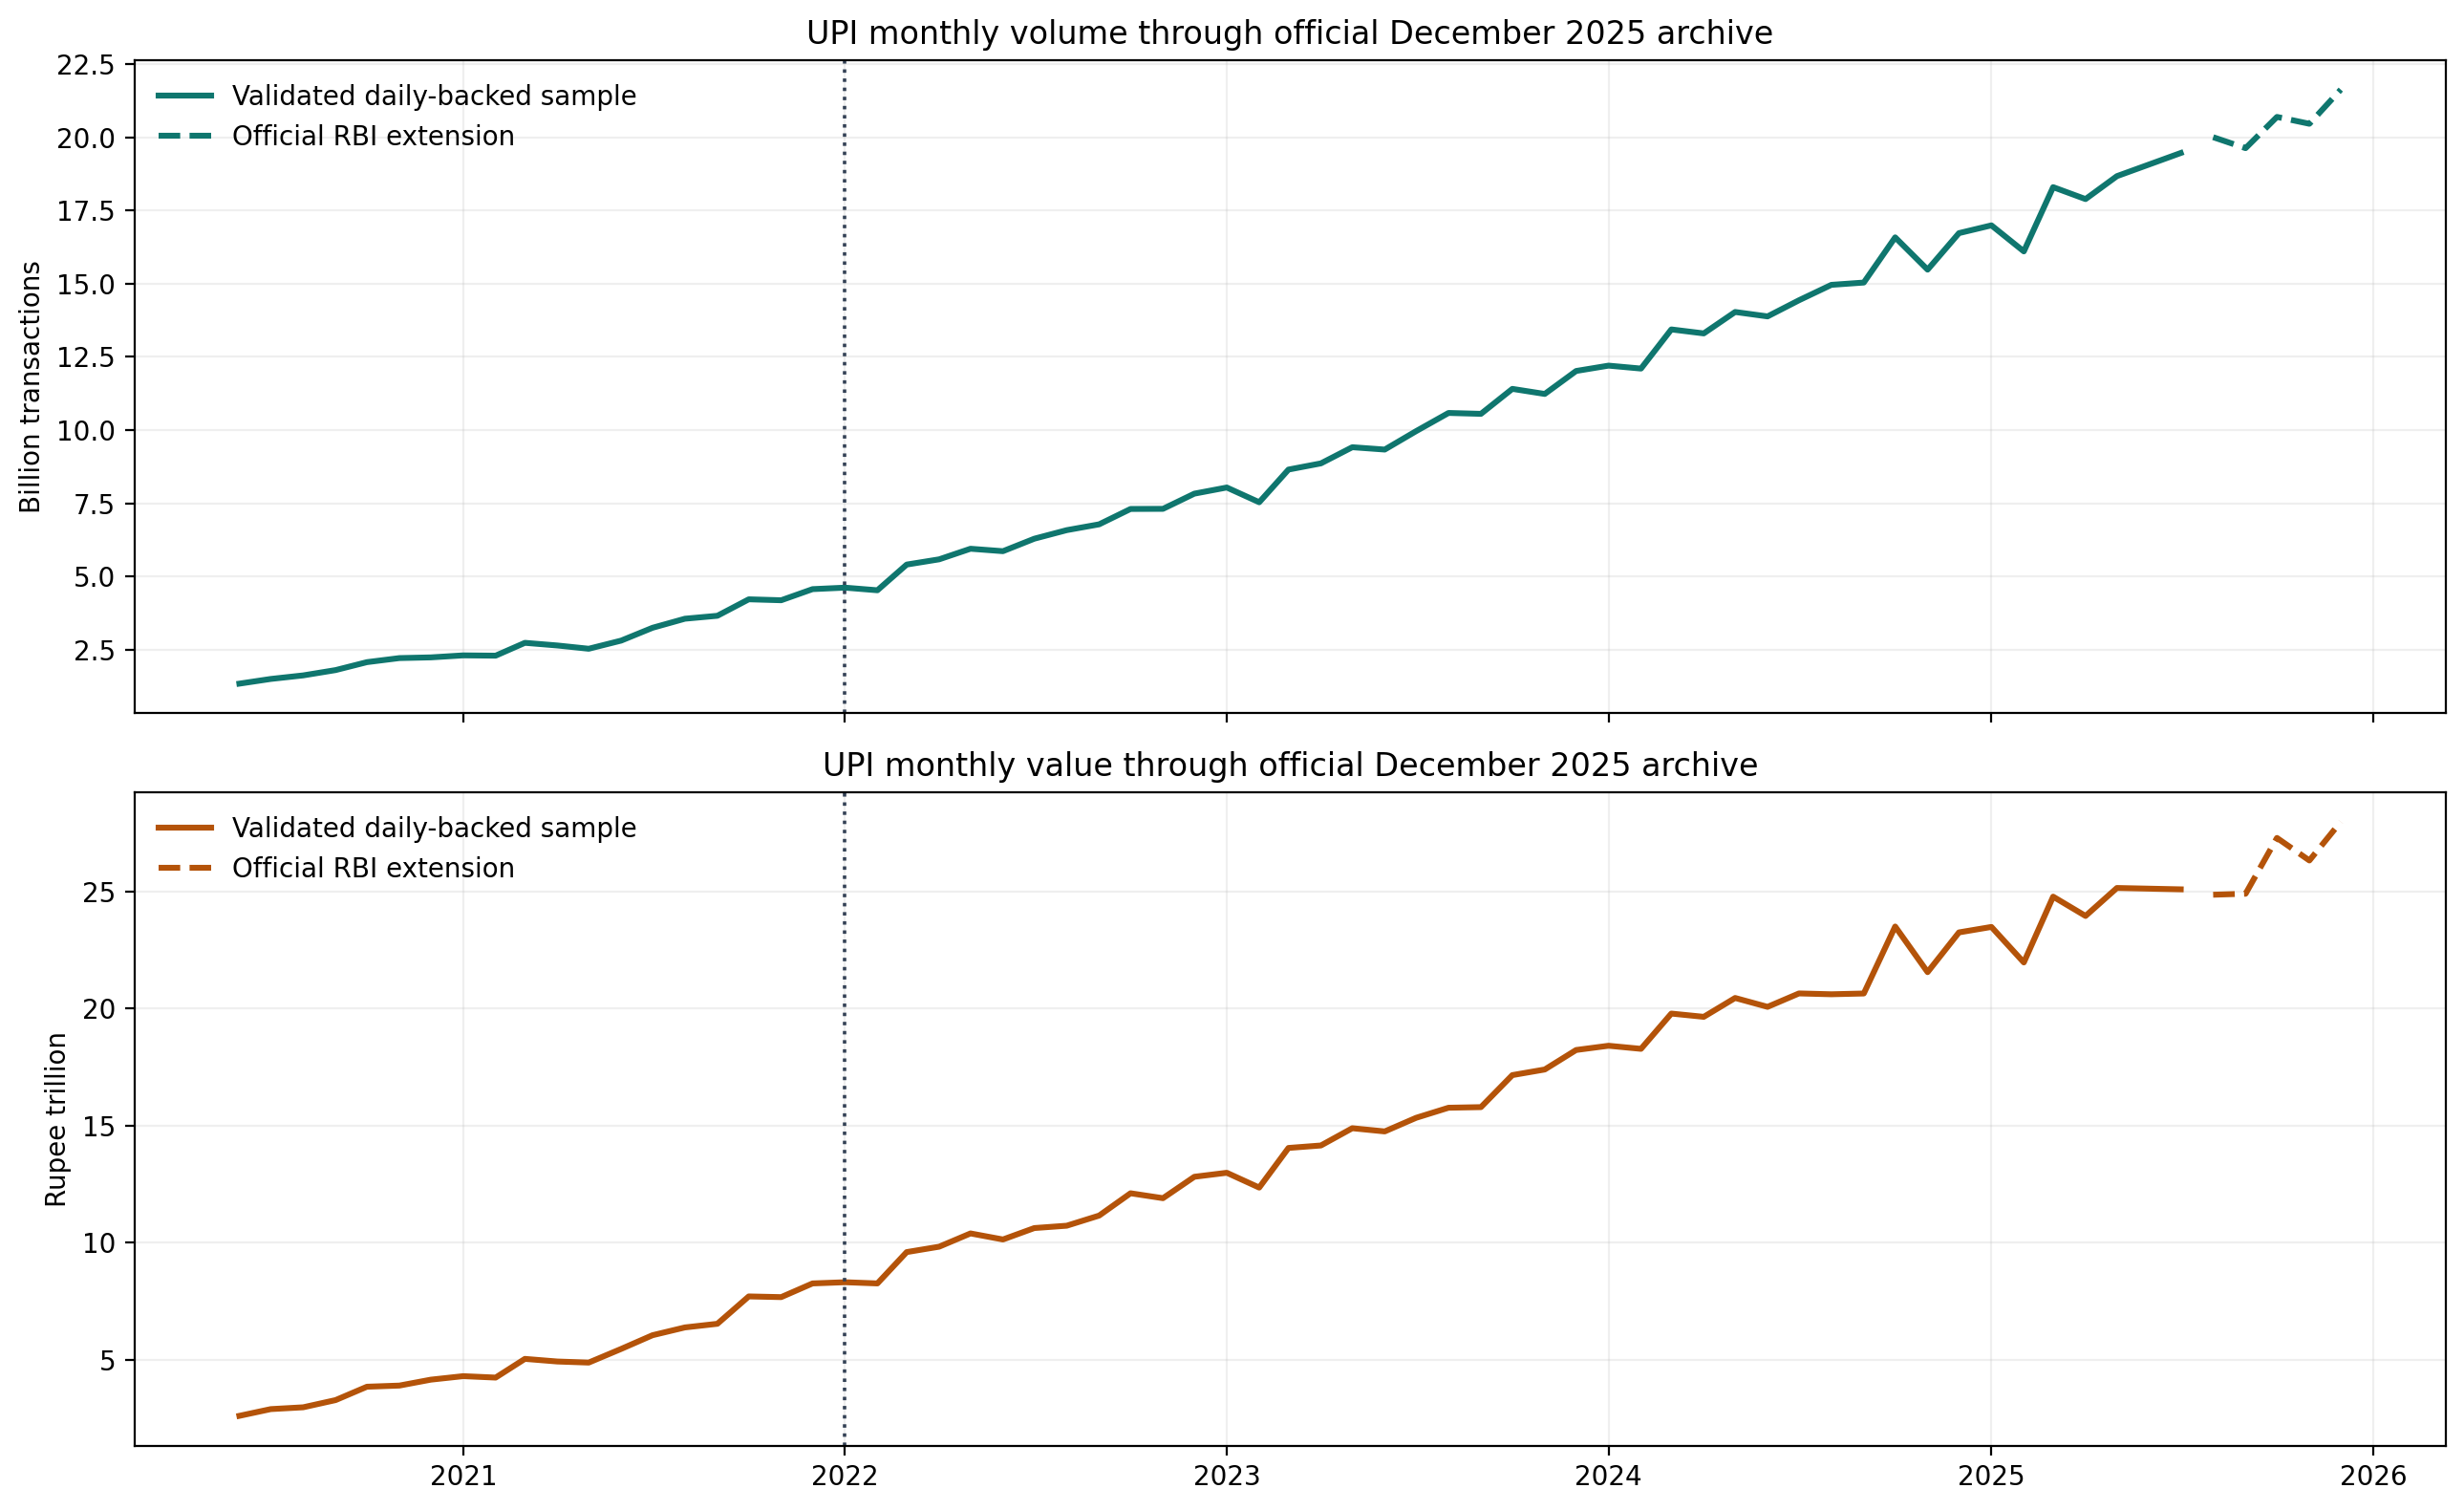
\includegraphics[width=\textwidth]{upi_plot_levels_extended.png}
\caption{Monthly UPI volume and value through the official December 2025 archive. The solid segment is backed by the validated daily panel; the dashed segment shows the official RBI monthly extension beyond July 2025.}
\label{fig:levels-extended}
\end{figure}

\section{Daily Data, Autocorrelation, and Annualised Robustness}

The daily panel adds high-frequency structure that the monthly series cannot show. Daily log-growth autocorrelations are:
\begin{table}[H]
\centering
\caption{Daily log-growth autocorrelation diagnostics}
\label{tab:daily-ac}
\small
\begin{tabular}{l c c}
\toprule
Series & Lag & Autocorrelation \\
\midrule
Daily log-growth in volume & 1 & -0.3865 \\
Daily log-growth in volume & 7 & 0.2170 \\
Daily log-growth in value & 1 & -0.3783 \\
Daily log-growth in value & 7 & 0.7033 \\
\bottomrule
\end{tabular}
\end{table}

The lag-7 dependence is especially strong for transaction value, pointing to meaningful weekly structure in payment activity. This is one reason HAC-robust inference is more appropriate than iid monthly assumptions.

Annualised averages reinforce the same story. Table~\ref{tab:annual} shows a steady slowdown in average monthly growth from 2021 through 2024.

\begin{table}[H]
\centering
\caption{Annualised average monthly growth}
\label{tab:annual}
\small
\begin{tabular}{c c c c}
\toprule
Year & Avg.\ monthly volume growth & Avg.\ monthly value growth & Complete year? \\
\midrule
2020 & 9.0277\% & 8.1647\% & No \\
2021 & 6.4091\% & 6.1157\% & Yes \\
2022 & 4.7332\% & 3.8411\% & Yes \\
2023 & 3.7748\% & 3.0769\% & Yes \\
2024 & 2.9148\% & 2.1933\% & Yes \\
2025 & 2.7282\% & 1.4604\% & No \\
\bottomrule
\end{tabular}
\end{table}

From a statistical-inference perspective, these annualised summaries are useful because they reduce short-run serial dependence. They should not replace the monthly analysis, but they do make the same qualitative point: the system keeps expanding, but at a lower percentage growth rate than in the early diffusion phase.

\begin{figure}[H]
\centering
\begin{minipage}[t]{0.49\textwidth}
\centering
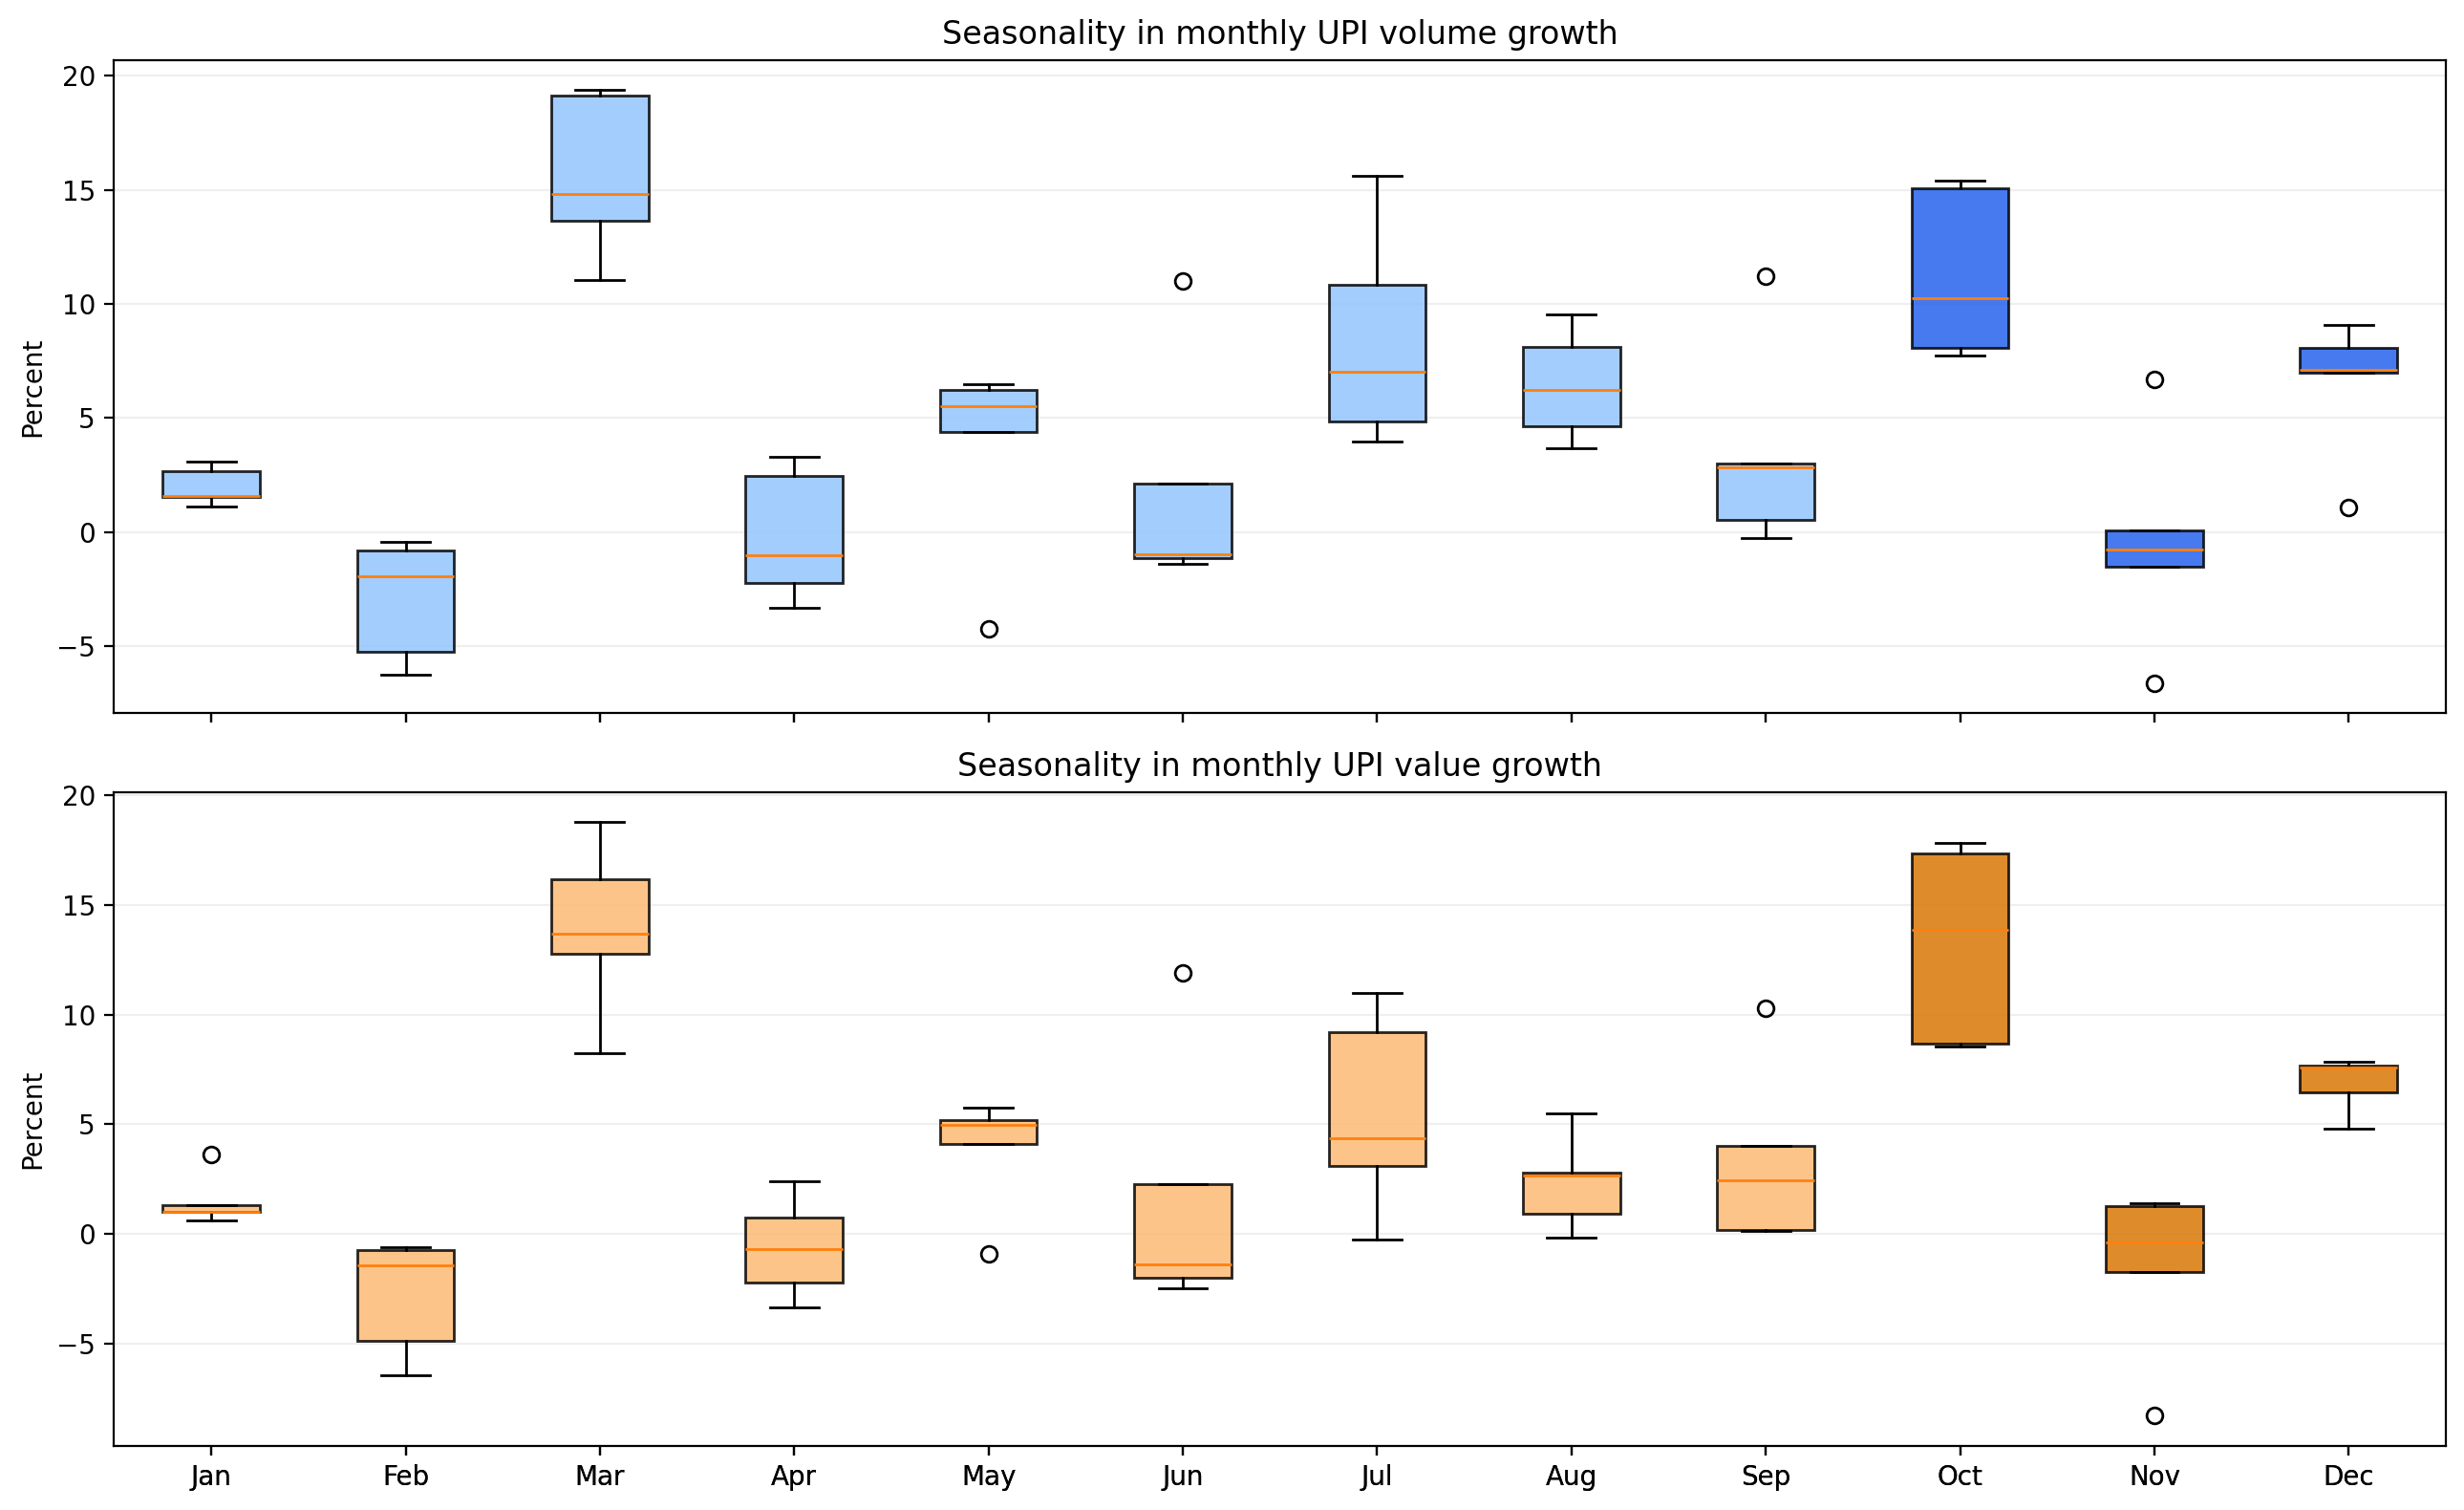
\includegraphics[width=\textwidth]{upi_plot_seasonality_boxplots.png}
\caption{Seasonality in monthly growth. October and December stand out more clearly in growth distributions than in the simple festival dummy tests.}
\label{fig:seasonality}
\end{minipage}\hfill
\begin{minipage}[t]{0.49\textwidth}
\centering
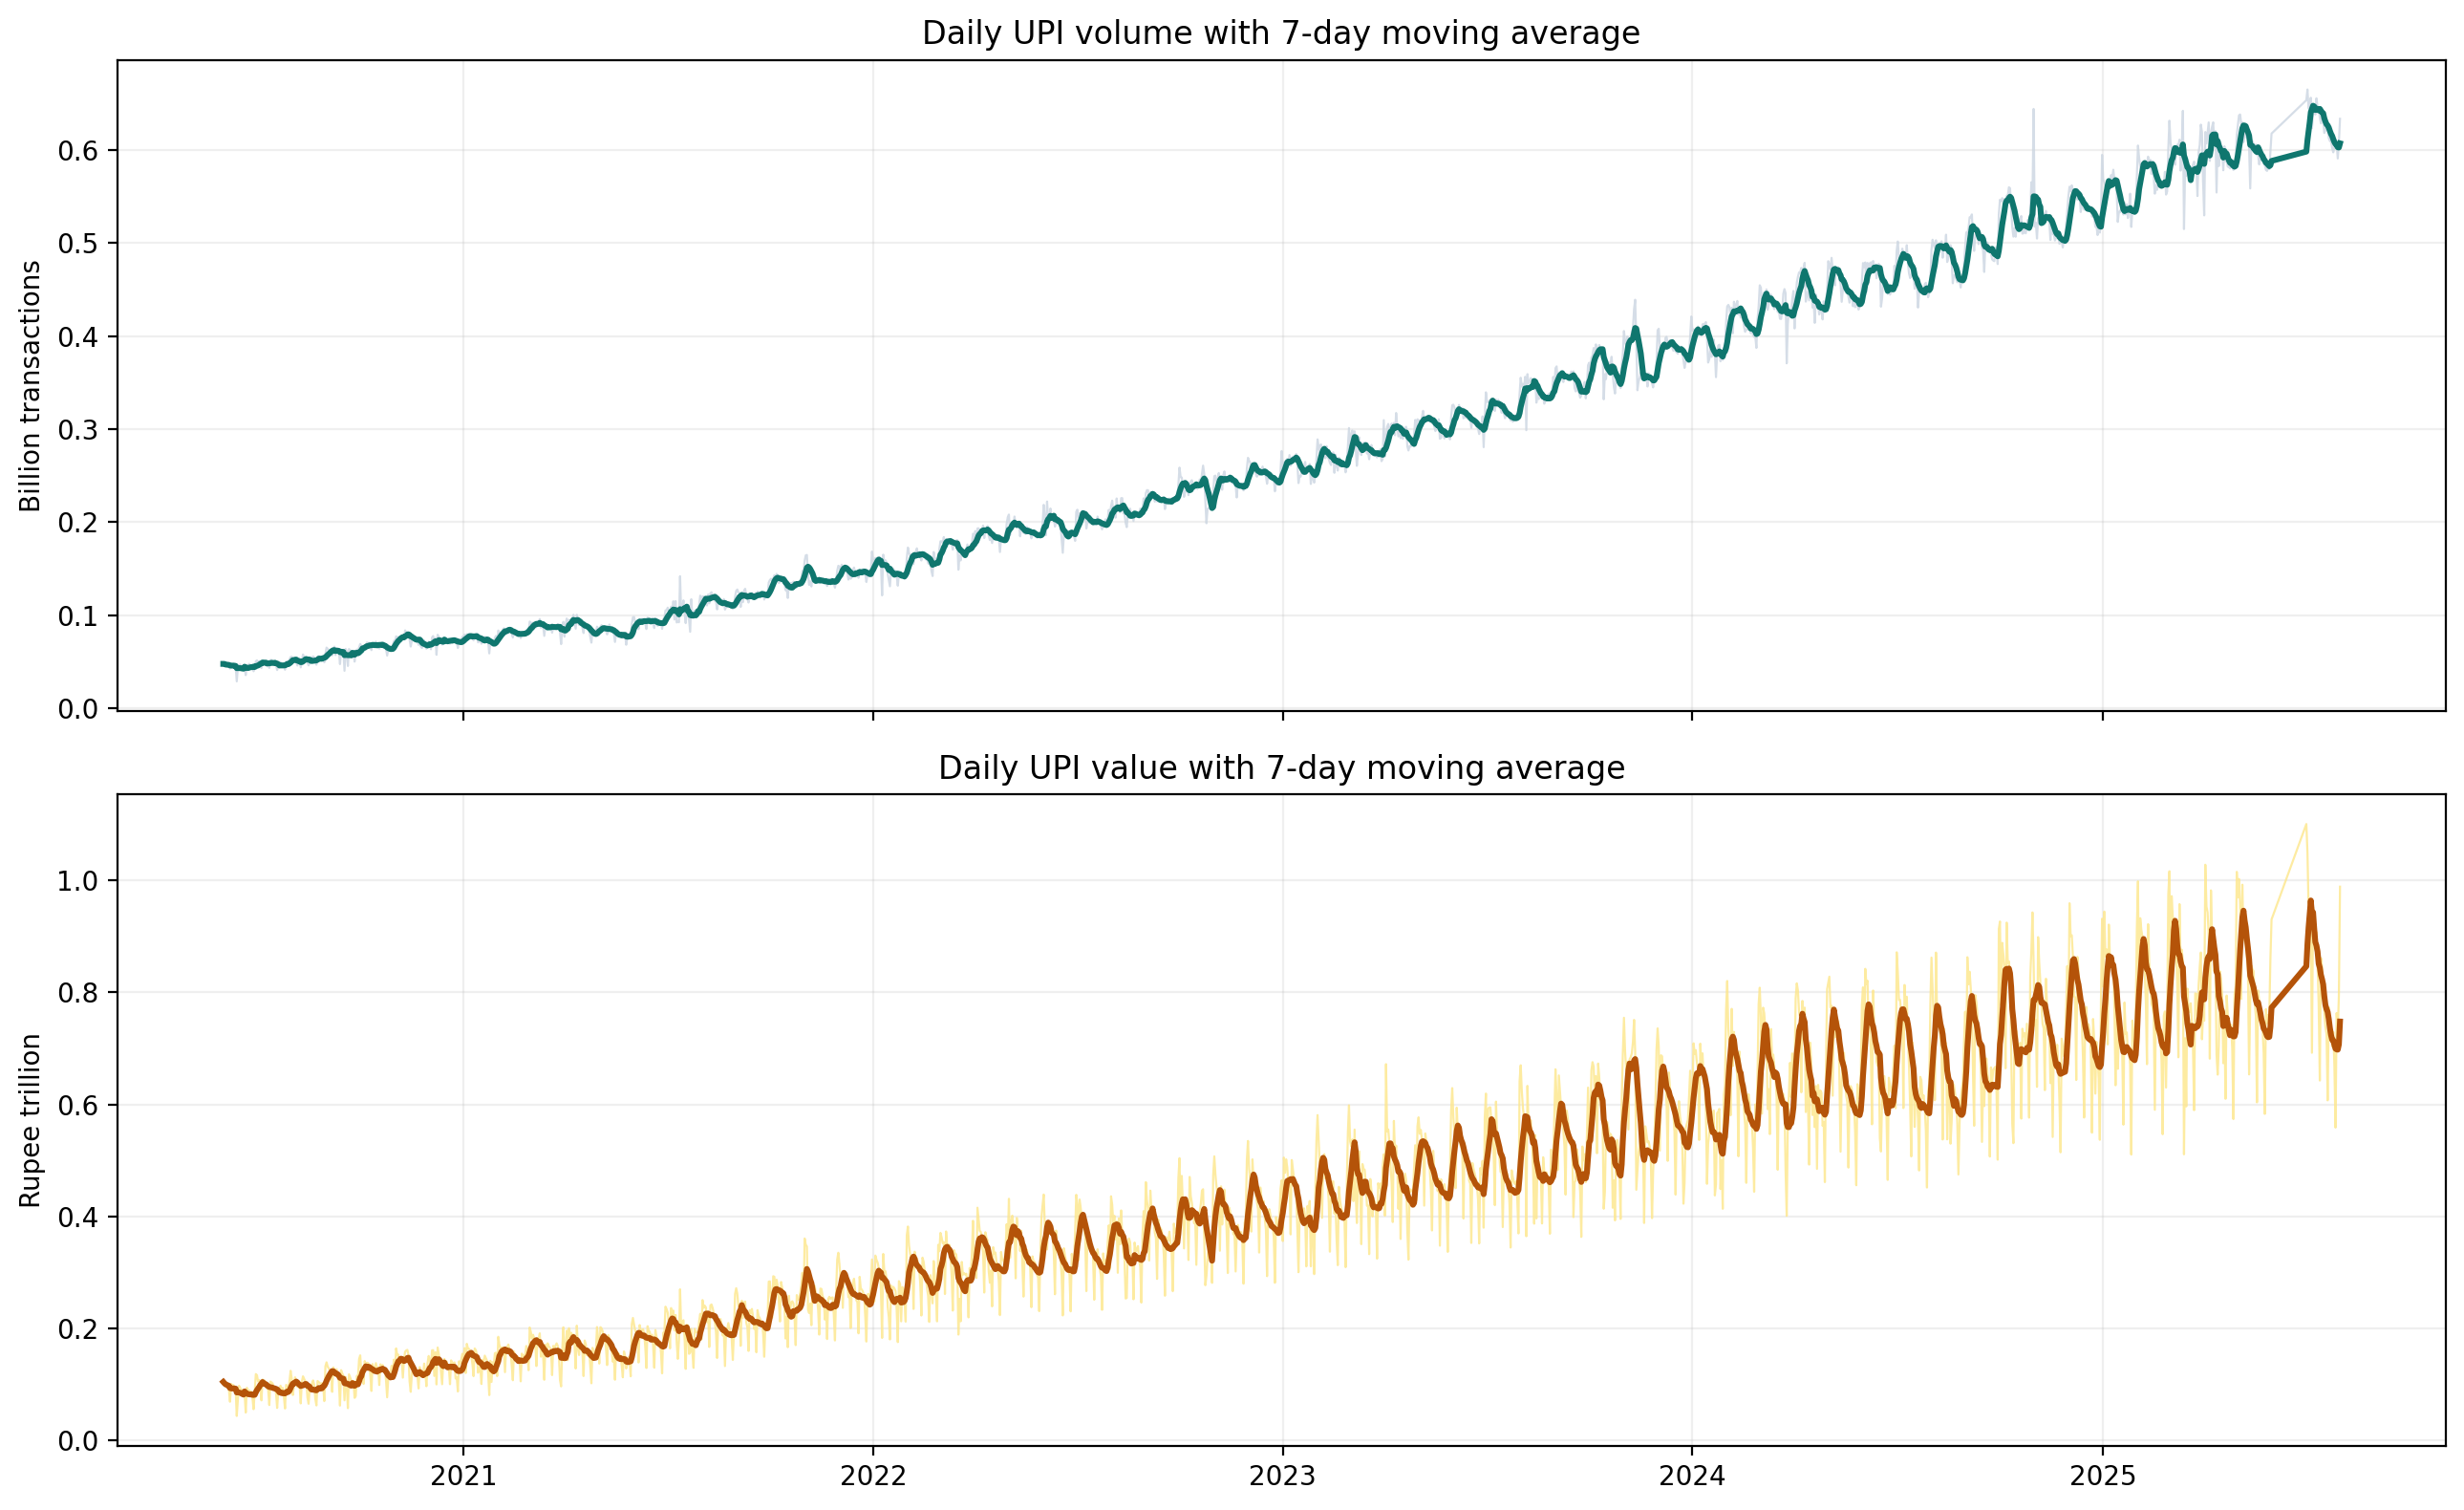
\includegraphics[width=\textwidth]{upi_plot_daily_trends.png}
\caption{Daily UPI volume and value with 7-day moving averages. The weekly structure in the daily series helps explain the need for autocorrelation-robust inference.}
\label{fig:daily-trends}
\end{minipage}
\end{figure}

\section{Interpretation and Practical Implications}

The correct summary is not that UPI is slowing in any literal usage sense. Rather, UPI is \emph{maturing}. On a very large base, smaller monthly percentage growth still implies massive absolute additions to transaction counts and value handled.

This matters operationally in at least three ways. First, capacity planning should focus on absolute load, not growth rates alone. A one-percentage-point change on a base above twenty billion monthly transactions still represents very large incremental demand on the payments stack. Second, fraud monitoring and resilience planning should account for concentrated risk windows, especially October and December, as well as weekly rhythms visible in the daily data. Third, interpretation should remain disciplined: lower growth is consistent with successful saturation and deep adoption, not necessarily with weakening digital-payments momentum.

\section{Limitations}

The daily panel ends in July 2025, so the main inference window ends there even though official monthly levels continue to December 2025. Festival measurement is intentionally simple and does not track movable-holiday timing precisely. The report is also descriptive-inferential rather than structural: it identifies statistically meaningful changes in growth behavior, but it does not model merchant adoption, policy interventions, or user heterogeneity directly.

\section{Conclusion}

This report answers the motivating question clearly. India's UPI story is no longer one of uniformly high percentage growth, but it is equally not a stagnation story. The data support a structural moderation in monthly growth rates after January 2022, while transaction levels continue to rise sharply. This is the signature of system maturity on scale. For an eight-page statistical inference report, the most defensible conclusion is therefore: \textbf{UPI is still growing strongly in levels, but the growth regime has changed.}

\section*{References}

\begin{enumerate}
  \item Reserve Bank of India. \emph{Payment System Indicators}. Available at: \url{https://www.rbi.org.in/Scripts/PSIUserView.aspx?Id=47}
  \item Reserve Bank of India. \emph{Database on Indian Economy}. Available at: \url{https://data.rbi.org.in}
  \item Press Information Bureau. \emph{UPI: Revolutionizing Digital Payments in India}. Available at: \url{https://www.pib.gov.in/PressReleaseIframePage.aspx?PRID=2079544}
  \item RBI-style daily payments datastore, resource id \texttt{1f9367ac-01b0-4c82-83a1-4069d4340667}, used only after validation against the official RBI monthly archive.
\end{enumerate}

\end{document}
